Initial efforts at WEC control optimization borrowed from wind and tidal energy control, which as shown, offers imperfect power capture.
The obvious contrast is that wind and tidal energy flows contain the majority of their energy in slowly-varying ``mean'' flows: though the frequency-domain characteristics of turbulence may be characteristically similar to wave spectra, they contain significantly less energy in viable wind/tidal/current energy sites, the fitness of which are determined primarily from the magnitude of the slowly-varying (i.e., hours to days) velocity components.
Consider this tidal cycle taken over 24 hours from a deployed acoustic doppler velocimeter in Admiralty Inlet, WA (\cite{NREL2015}, \figurename~\ref{fig: TidalVelocity}).

\begin{figure}
	\centering 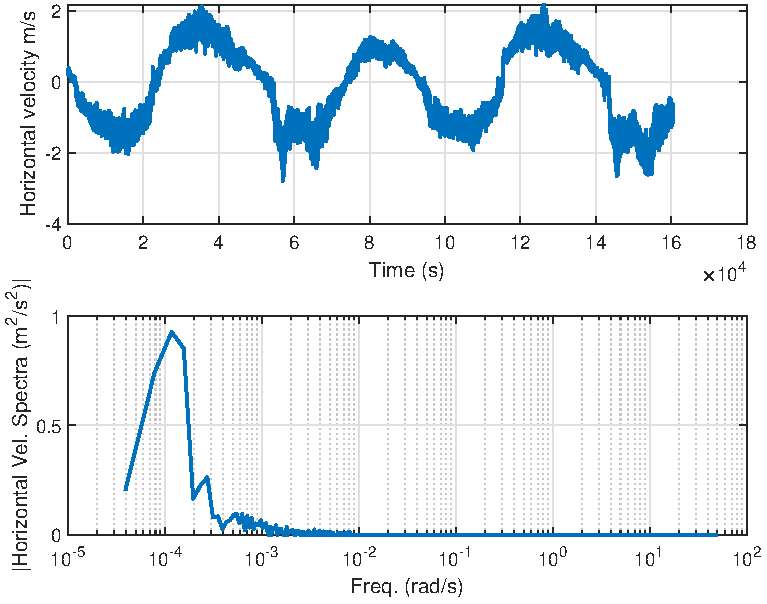
\includegraphics[width=\columnwidth]{TidalVelocity.pdf}
	\caption{Acoustic doppler velocimeter data from an approximately 45 hour deployment in Admiralty Inlet, WA.
	Sampled at 16 Hz.}
	\label{fig: TidalVelocity}
\end{figure}

However, a wind/tidal turbine can be similarly decomposed into a transfer function representation as per \figurename~\ref{fig:wec_as_multiport_block_diagram}, where the wind/water speed $U$ exerts a torque on the rotor $\tau_h$ which is summed with a controller torque $\tau_{pto}$, and the intrinsic impedance of the rotor and drivetrain are

\begin{subequations}
		
	\begin{gather}
		Z_{turb,i}(\omega)=b_f + j\omega J_{turb} \\
		Z_{turb,d}(\omega)=b_d + j\omega J_d
	\end{gather}
\end{subequations}

\noindent{respectively, and the motor/generator impedance is described as \ref{eq:winding_impedance}.
Note that the excitation force exerted from fluid velocity $U$, is a non-linear function, but may be approximated as linear over small perturbations.
While representing a non-linear rotor system as a first-order transfer function is an abstraction, it is a useful model when one considers that a family of first-order models linearized about different rotor operating points could reasonably approximate overall system dynamics, and each of those first-order models will be characteristically similar to those presented here: these conclusions are at least qualitatively valid over stable rotor operating states.
	
Considering the rotor itself, a gearbox, internal drivetrain components, and a motor/generator, the wind/tidal turbine system can also be described as the two-port networks in \figurename~\ref{fig:wec_as_multiport_circuits}.
Following the derivations in the the preceeding sections we arrive again at the following bi-conjugate impedance matching conditions expressed in Equations \eqref{eq:expanded_zin} and \eqref{eq:expanded_zout}}.
Considering $Z_L$, we again aim to maximize electrical power delivered to the load (i.e., ``Region 2 control'' \cite{Handbook2011}), and to preserve generality we consider feedback controllers of the form above (Eq.
\ref{eq:pi_controller_structure}), in which $\tau_{pto}$ is determined from a measurement rotor angular velocity $\omega$.
These conditions are plotted using parameters summarized in Table \ref{tab:tidal phyiscal_params} in \figurename~\ref{fig: RotorZinZout}.


\begin{table}[tb]
	\caption{Parameters of the hypothetical tidal power system.}
	\label{tab:tidal phyiscal_params}
	\centering
	
	\begin{tabular}{rc}
		\hline
		
		\hline
		\textbf{Parameter} & \textbf{Value} \\
		\hline
		Rotor friction $b_f$ [Nm\_s/rad] & 1 \\
		Rotor inertia $J_{turb}$ [kg-m$^2$] & 10 \\
		Gear ratio, $N$ [rad/rad] & 12.4666 \\
		Shaft inertia, $J_d$ [kg\,m$^2$]                & 1 \\
		Shaft friction, $b_d$ [Nm\,s/rad]               & 0.1 \\
		Torque constant, $k_\tau$ [Nm/A]                & 6.1745 \\
		Motor winding resistance, $R_w$ [$\Omega$]      & 0.1 \\
		Motor winding inductance, $L_w$ [H]             & 0.1 \\
		\hline
		
		\hline
	\end{tabular}
\end{table}

\begin{figure}
	\centering 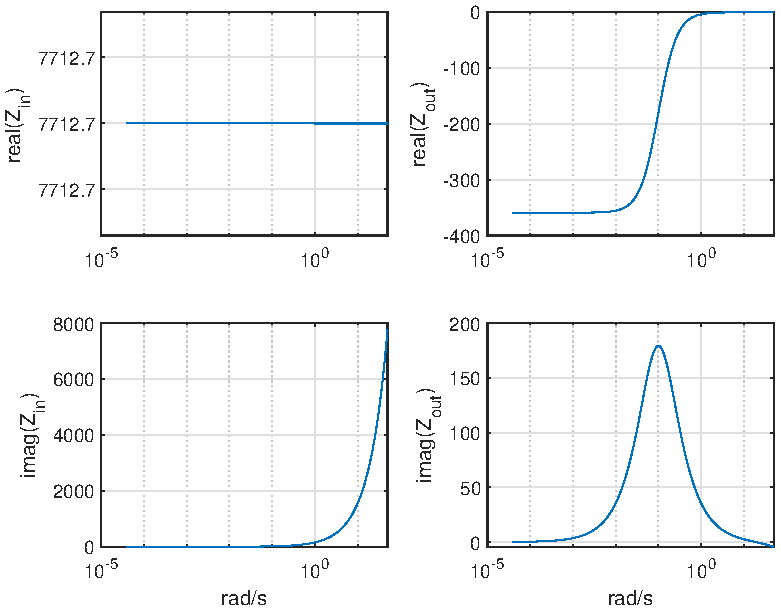
\includegraphics[width=\columnwidth]{RotorZinZout.pdf}
	\caption{Real (top) and imaginary (bottom) parts of the input (left) and output (right) impedance.}
	\label{fig: RotorZinZout}
\end{figure}

The key characteristic difference in the appearance of the input and output impedances is the absence of a stiffness-type term in the intrinsic and drivetrain impedances, implying that these are now first-order systems.
Note that over the energy-containing frequencies of the flow, that the imaginary part of both $Z_{in}$ and $Z_{out}$ are zero, implying that a damping-type controller will be optimal over these frequencies \eqref{eq:bi_conj_matching_out} and that the co-design problem is the proper selection of $N$ and $K_T$ and the minimization of friction losses $B$ and $B_d$ \eqref{eq:bi_conj_matching_in}, \eqref{eq:bi_conj_matching_out}.
Though co-design for wind/tidal rotors is not typically formalized in this way, note that the common wind turbine control algorithm $\tau_{pto} = K\omega^2$, where $K$ is a constant determined from the aerodynamic parameters of the rotor, is effectively a non-linear damper for which there is no reactive control term.
Further, towards higher frequencies where the imaginary part of $Z_{out}$ increases, the optimal controller will need positive phase (e.g., a lead compensator) to capture any excitation present at these frequencies: in fact, state-of-the-art wind turbine controllers use an ``upstream'' measurement or model of accelerations in free-stream velocity and adjust rotor state ahead of time to maximize power capture of the stochastically varying free-stream turbulence \cite{Schlipf2013b}.
Under these conditions, bi-conjugate impedance matching conditions become increasingly relevant, but are still not commensurately critical as their application to wave energy where the vast majority of the available energy is not contained in a ``steady'' mean flow (or one that varies at frequencies much lower than the device dynamics).

Considering the selection of $N$ and $K_T$ values, the appropriate gear ratio is more probably driven by the combined consideration of 1) an efficient generator operating speed and torque and 2) the designed tip-speed ratio of the rotor (and its implied $\omega$ in a given $U$).
If the non-linear fluid excitation of the rotor is taken as guidance in these design decisions, which over excited frequencies affects the real part most significantly, then bi-conjugate impedance matching conditions simplify further to the minimization of friction losses $B$ and $B_d$.

In this way, we see that the underlying theory is, with some linearizing approximations, valid for the power capture of wind/tidal turbines as well, but bi-conjugate impedance matching conditions are simpler to achieve over the energetic frequency bands and historically did not need to be considered explicitly for efficient energy capture because the frequency ranges over which device and PTO dynamics become important tend to be significantly higher.
Secondly, the nonlinearities of the aerodynamic system lead to more convenient power-maximizing control formulations in the time-domain.
